\begin{tikzpicture}
  % corps A
  \tikzCercle[gray!50!white] (0, 0) {20}
  \tikzLabel*(-1.2, 0) {$m_A$}
  \tikzLabel(0,0) {$A$}
  % corps B
  \tikzCercle[gray!50!white] (4, 2) {20}
  \tikzLabel*(2.8, 2) {$m_B$}
  \tikzLabel(4, 2) {$B$}
  % force et distance
  \tikzVecteur(4, 2) (-1.75, -0.875) {$\vvFAsurB$} [left]
  \tikzVecteur*(0.5, -1) (4, 2) {}
  \tikzLabel*(2.5, -0.5) {$d$}
\end{tikzpicture}